\documentclass[11pt,a4j,fleqn]{jarticle}
\usepackage{amsmath,amsthm,amssymb}
\usepackage[dvipdfmx]{graphicx}

\title{課題2}
\author{花嶋陽}
\date{6/2}


\begin{document}

\maketitle

\section{はじめに}



\section{包絡線定理}

包絡線定理の解説を書く.

数式(番号なし)の例
\[
f(x, t) = t x - t^2
\]


数式(番号つき)の例
\begin{equation}
f(x, t)  = -(t - \frac{x}{2})^2 + \frac{x^2}{4} \label{eq:square}
\end{equation}

数式(番号つき)の例(高さが調整されたカッコ)
\begin{equation}
f(x, t) = -\left(t - \frac{x}{2}\right)^2 + \frac{x^2}{4} \label{eq:square-2}
\end{equation}



数式番号の引用の例:
平方完成の式\eqref{eq:square}より...

\begin{figure}
 \centering
 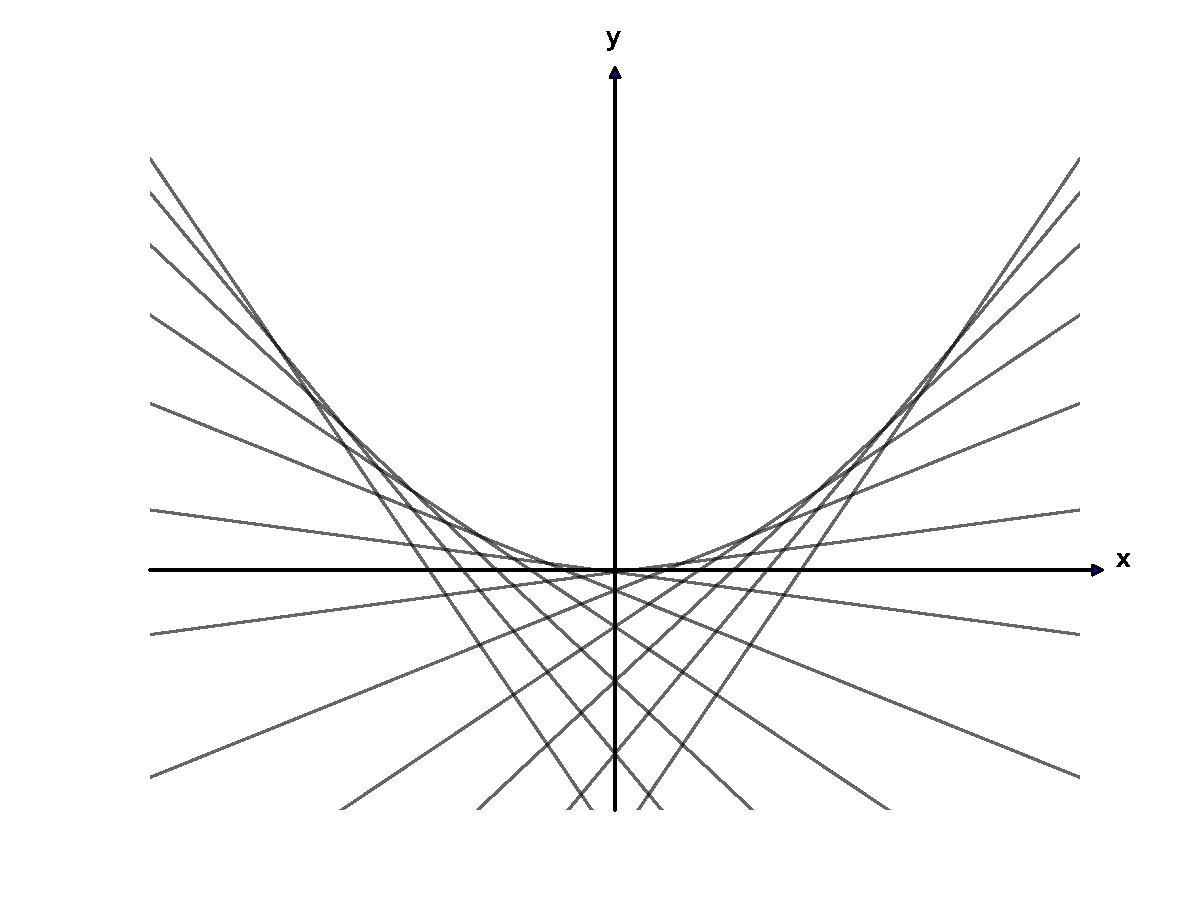
\includegraphics[scale=0.5]{envelope0.pdf}
 \caption{1つ目の図の表示}
 \label{fig:1}
\end{figure}

\begin{figure}
 \centering
 \includegraphics[scale=0.5]{envelope1.pdf}
 \caption{2つ目の図の表示}
 \label{fig:2}
\end{figure}



引用の例:尾山・安田\cite{OyamaYasuda11}.


\subsection{サブセクションのタイトル}

必要ならサブセクションを作る.



\section{Pythonプログラム}

自分のPythonプログラムの説明を書く.

コードの表示の例
\begin{quote}
\begin{verbatim}
import numpy
from matplotlib import pyplot
x = numpy.arange(0, 10, 0.1)
y = numpy.cos(x)
pyplot.plot(x,y)
pyplot.show()
\end{verbatim}
\end{quote}

\verb|\begin{verbatim}| ... \verb|\end{verbatim}| の中では改行は自動ではされない.
長すぎてページからはみ出す行は自分で適宜改行する.



\begin{thebibliography}{0}
\bibitem{OyamaYasuda11}
尾山大輔・安田洋祐「経済学で出る包絡線定理」『経済セミナー』2011年10・11月号.
\end{thebibliography}

\end{document}